\subsection{Neural Networks}

One of the best online resources I've discovered for understanding neural networks is from Michael Nielson. He's written an online textbook called "Neural Networks and Deep Learning" that can be found at \url{http://neuralnetworksanddeeplearning.com}. My notes and notation below are mainly based off of his chapter 2 for understanding the math behind neural nets. I've also included some notes from the Deep Learning book by Ian Goodfellow, Yoshua Bengio, and Aaron Courville.
 
To help visualize these concepts, I've diagrammed a basic neural network in figure \ref{fig:neural_net_image}. The general idea of these networks is to pass in the original features $x_1$ and $x_2$ for example, as weighted linear combinations into the different nodes within the first layer. The first layer in this example has only two nodes. So for node 1 we pass in the linear combination:
\begin{equation}
x_1w^{(1)}_{11} + x_2w^{(1)}_{12}  + (1)b^{(1)}_1.
\end{equation}
 
\begin{figure} \label{fig:neural_net_image}
\caption{Example of a two layer neural network}
\centering
 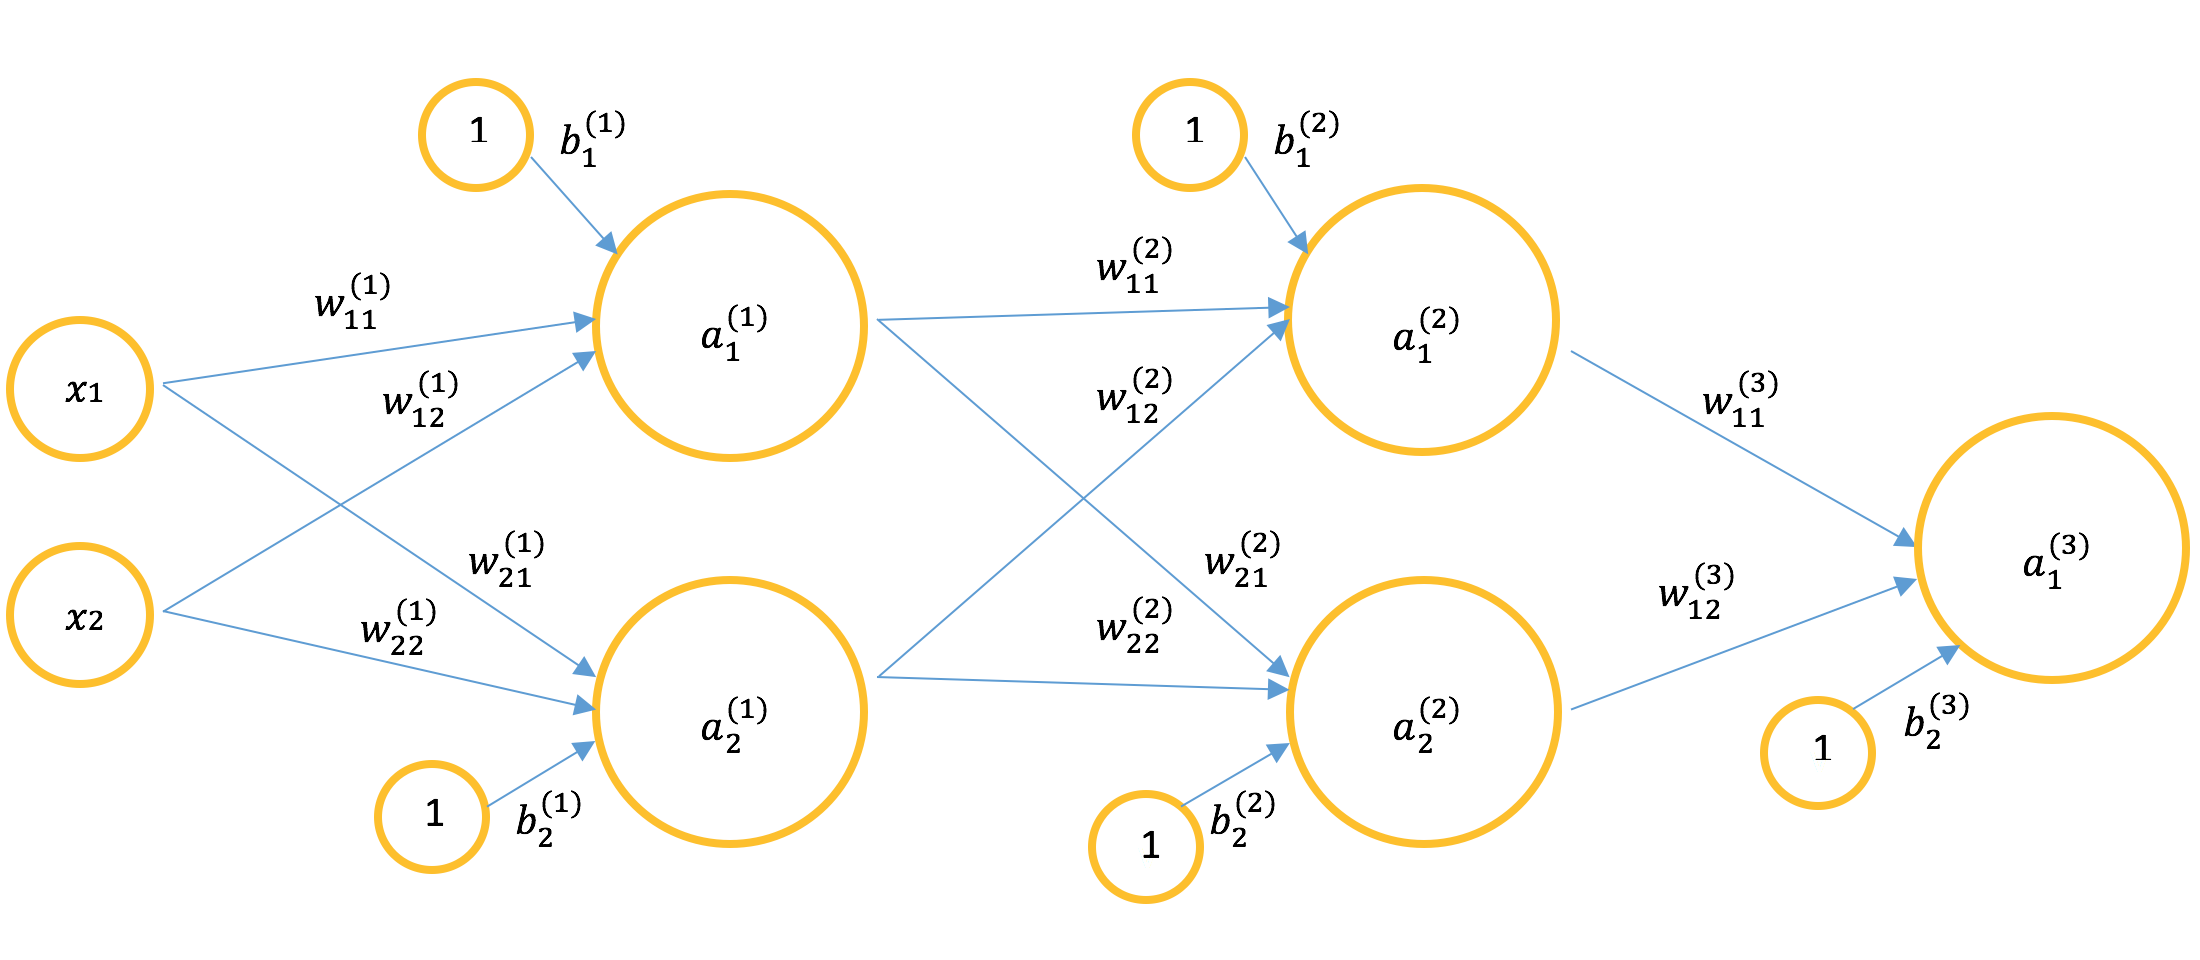
\includegraphics[scale=.3]{neural_net_image.png}
 \end{figure}
 
The notation here is important to keep straight. For the weights the number in the superscript is referring to the current layer, the first number in the subscript is referring to which node the previous node output (or feature) is going to, and the second number in the subscript is referring to which node (or feature) the current weight is coming from. So for example, $w^{(1)}_{12}$ is a weight in the first layer (because of the superscript) and connects the second feature to the first node. 

This notation comes from Nielson's book and helps when we write everything out in matrix multiplication. To see what that looks like for a given layer:

\[
\begin{bmatrix}
           z^{(1)}_{1} \\
           z^{(1)}_{2} \\
           \vdots \\
           z^{(1)}_{m}
         \end{bmatrix}
         =
\left[
  \begin{array}{cccc}
    w^{(1)}_{11} & w^{(1)}_{12} & \hdots & w^{(1)}_{1n} \\
    w^{(1)}_{21} & w^{(1)}_{22} & \hdots & w^{(1)}_{2n} \\
    \hdots &  \hdots  & \hdots &  \hdots \\
    w^{(1)}_{m1} & w^{(1)}_{m2} & \hdots & w^{(1)}_{mn} \\ 
  \end{array}
\right]
\begin{bmatrix}
           x_{1} \\
           x_{2} \\
           \vdots \\
           x_{n}
         \end{bmatrix}
+
\begin{bmatrix}
           b^{(1)}_{1} \\
           b^{(1)}_{2} \\
           \vdots \\
           b^{(1)}_{m}
         \end{bmatrix}
\]

\noindent where $n$ is the number of features, $m$ is the number of nodes, and the $z$'s are the weighted combinations. In shorthand we can write:

\begin{equation}
\mathbf{z}^{(1)} = \mathbf{W}^{(1)} \mathbf{x} + \mathbf{b}^{(1)}.
\end{equation}

One other note to make here is that the bias ($b^{(1)}$) essentially just provides a constant in our linear combination since we are only multiplying it by 1. 

Once this linear combination is fed into the node we pass it through what is known as an activation function. The purpose of this is to help our neural net model nonlinear behavior (see Deep Learning book for further discussion, pages 168-171). We represent the activation function with $\sigma$ and write the output of the activation function as:
%TODO talk about activation functions here

\begin{equation}
\mathbf{a}^{(1)} = \mathbf{\sigma}(\mathbf{W}^{(1)} \mathbf{x} + \mathbf{b}^{(1)}) = \sigma(\mathbf{z}^{(1)})
\end{equation}
\noindent As Nielson points out we are treating the function $\sigma$ here as a vectorized function. A more explicit way to write this out would be:

\[
\begin{bmatrix}
           a^{(1)}_{1} \\
           a^{(1)}_{2} \\
           \vdots \\
           a^{(1)}_{m}
         \end{bmatrix}
         =
\left[
  \begin{array}{cccc}
    \sigma(w^{(1)}_{11}x_1 & w^{(1)}_{12}x_2 & \hdots & w^{(1)}_{1n}x_n + b_1^{(1)}) \\
    \sigma(w^{(1)}_{21}x_1 & w^{(1)}_{22}x_2 & \hdots & w^{(1)}_{2n}x_n + b_2^{(1)} ) \\
    \hdots &  \hdots  & \hdots &  \hdots \\
    \sigma(w^{(1)}_{m1}x_1 & w^{(1)}_{m2}x_2 & \hdots & w^{(1)}_{mn}x_n + b_m^{(1)} ) \\ 
  \end{array}
\right]
\]

To continue this notation with each subsequent layer we really only need to change a few things. First of all, instead of the original features $x_1, x_2, ..., x_n$ we have $a^{(1)}, a^{(2)}, ..., a^{(m)}$ as the inputs into the next layer. This leads us to change our weight matrix as well so that we have a matrix that is $p$x$m$ where $p$ is the number of nodes in the second layer and $m$ is the number of outputs from layer 1 (before we had $n$ representing the number of \emph{features}). The other thing we need to change is the superscript for the variables such as $\mathbf{W}^{(1)}$ to $\mathbf{W}^{(2)}$ since we are in the second layer. For a generic layer from Nielson's book we can write:

\begin{equation}
\mathbf{z}^{(l)} = \mathbf{W}^{(l)} \mathbf{a}^{(l-1)} + \mathbf{b}^{(l)}.
\end{equation}
\noindent This leads us to also write:

\begin{equation}
\mathbf{a}^{(l)} = \mathbf{\sigma}(\mathbf{z}^{(l)}).
\end{equation}


 
 Now that we have our notation straight we can talk about how the network is trained. Really at the heart of the backprop algorithm is gradient descent or some iterative optimization technique. To use gradient descent or similar techniques we need to calculate the derivatives of the cost function with respect to the parameters in the model or in the case of neural networks, the weights and biases. Because the neural network is made up of different layers or functions then what this amounts to is using the chain rule for each parameter.
 
 Using our example and notation, lets find the derivative of the cost function with respect to the weight $w^{(1)}_{12}$ for example. In other words we want to find:
 
 \begin{equation}
\frac{dC}{dw^{(1)}_{12}}.
 \end{equation}
 
\noindent A common loss function is the squared-error loss function or:
 
 \begin{equation}
 C = \frac{1}{2} {(y_i - a_1^{(3)})^2}
 \end{equation}
 
 \noindent where $a_1^{(3)}$ is the output from the last layer in our example. Note that we are doing this for one particular training example which we'll talk about later.
 %TODO talk about this later!
 
 To get at the derivative for $w^{(1)}_{12}$ we rewrite the cost function above with all its nested functions:
 
 \begin{equation}
 \begin{split}
 \frac{1}{2} (y_i - a_1^{(3)})^2 & = \frac{1}{2} (y_i - \sigma(w^{(3)}_{12}a_2^{(2)} + w^{(3)}_{11}a_1^{(2)}+ b_2^{(3)}))^2 \\
 &= \frac{1}{2} (y_i - \sigma(w^{(3)}_{12} \sigma(w^{(2)}_{22}a_2^{(1)} + w^{(2)}_{21}a_1^{(1)}+ b_2^{(2)}) + w^{(3)}_{11}        \sigma(w^{(2)}_{12}a_2^{(1)} + w^{(2)}_{11}a_1^{(1)}+ b_1^{(2)}) + b_2^{(3)}))^2 \\
 &= \frac{1}{2} (y_i - \sigma(w^{(3)}_{12}     \sigma(w^{(2)}_{22}   \sigma(w_{22}^{(1)}x_2 + w_{21}^{(1)}x_1 + b_2^{(1)})    + w^{(2)}_{21}        \sigma(w_{12}^{(1)}x_2 + w_{11}^{(1)}x_1 + b_1^{(1)})+ b_2^{(2)}) \\
 &+ w^{(3)}_{11}        \sigma(w^{(2)}_{12}  \sigma(w_{22}^{(1)}x_2 + w_{21}^{(1)}x_1 + b_2^{(1)})  + w^{(2)}_{11} \sigma(w_{12}^{(1)}x_2 + w_{11}^{(1)}x_1 + b_1^{(1)})+ b_1^{(2)})     + b_2^{(3)}))^2
 \end{split}
 \end{equation}

We then use the chain rule to get:

\begin{equation}
\frac{dC}{dw^{(1)}_{12}} = (y_i - a_1^{(3)})(-\sigma^\prime(z_1^{(3)}))[w_{12}^{(3)}\sigma^\prime(z_2^{(2)})w_{21}^{(2)}\sigma^{\prime}(z_1^{(1)})x_2 + w_{11}^{(3)}\sigma^{\prime}(z_1^{(2)})w_{11}^{(2)}\sigma^{\prime}(z_1^{(1)})x_2].
\end{equation}

 %TODO everything above is good for publishing
Finding all partial derivatives with respect to our parameters, such as the weights and biases, gives us our gradient $\nabla C$ which is used in the gradient descent equation:

\begin{equation}
\theta_t = \theta_{t-1} + \eta \left( -\nabla C(\theta_{t-1}) \right).
\end{equation}
In this equation $\theta_t$ represents the parameters to the neural network at iteration $t$, $C$ represents our cost function, and $\eta$ is the learning rate. In the example above we used the squared-error loss for the cost function which in general form is given by:

\begin{equation}
C(\theta) = \frac{1}{2}(y_i - f_\theta(x_i))^2.
\end{equation}
\noindent where $f$ is the neural network, $\theta$ represents the parameters of the network (the weights and biases) and $x_i, y_i$ represent the $i^{th}$ training pair. It is key to remember that we are treating this loss function as a function of $\theta$ and keeping everything else fixed. The goal is to find the $\theta$ that minimizes the loss function.





\subsection{Backprop}
As we can see from the previous section, the algebra for this can get lengthy and messy. 

\begin{equation}
\frac{dC}{dw^{(1)}_{12}} = a_{2}^{0}\delta_1^{(1)}
\end{equation}

The quantity $\delta_1^{(1)}$ is given by:

\begin{equation}
(w_{11}^{(2)}\delta^{(2)}_1 + w_{21}^{(2)}\delta^{(2)}_2)\sigma^{\prime}(z_1^{(1)})
\end{equation}
 
 We then recursively get the other $\delta$'s in the equation:
 
 \begin{equation}
 \begin{split}
 \delta^{(2)}_1  & = w_{11}^{(3)}\delta_1^{(3)}\sigma^{\prime}(z_1^{(2)})\\
 \delta^{(2)}_2  & = w_{12}^{(3)}\delta_1^{(3)}\sigma^{\prime}(z_2^{(2)})
 \end{split}
 \end{equation}
 

 
 
 For me, the best way to understand how a neural net works is to look at an actual network and learn by example. One of the classic examples is the XOR function. A discussion of this problem can be found in the Deep Learning book on pg. 167.

Figure \ref{fig:xor} shows what the data looks like for this problem. We have two features, $x_1$ and $x_2$, that can take on two possible values, 0 or 1. We assign another binary variable $y$ to each of the possible combinations of $x_1, x_2$ resulting in $(0,0) = 0, (0,1)=1, (1,1)=1, (1,0)=0$.

The goal here is to find a line that separates the response variable $y$ between its two possible values, 0 or 1. As we can see from the picture this is not possible with the current setup.

 \begin{figure} \label{fig:xor}
\caption{XOR problem}
\centering
 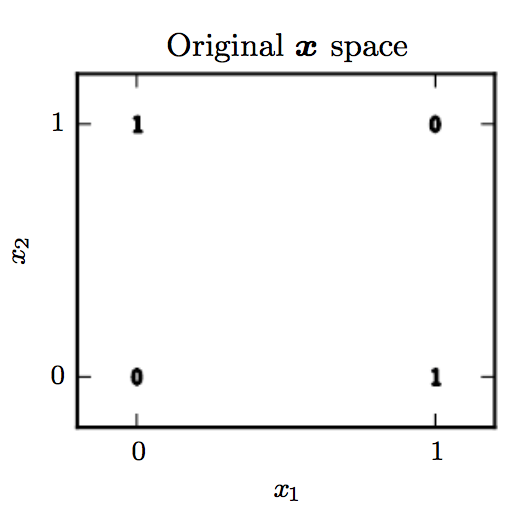
\includegraphics[scale=.7]{xor.png}
 \end{figure}
 